% 图 49.2 —— 由 `checks/emit_hand.py` 自动拼出（probe 精测 + prims2 图元分解）
%%
% ⚠ 这是**稿子不是成品**：跑 `checks/checkhand.py 49.2` 看指标 + 看叠合图。
%%
%% ⚠ 待核：
%   · 本图 probe 报出阴影族 1 个 —— **本脚本不生成阴影**（要照原书手写）；prims2 的 strokes 里可能含阴影线，核对时留意别画重
%   · 可疑字形 1 项（空心圈 ⊙ 常被认成字母 o）—— 见文件末
%%
\documentclass[12pt]{standalone}
\usepackage{fontspec}
\setsansfont{Arial}
\newfontfamily\mfallback{DejaVu Sans}
\usepackage{tikz}
\begin{document}
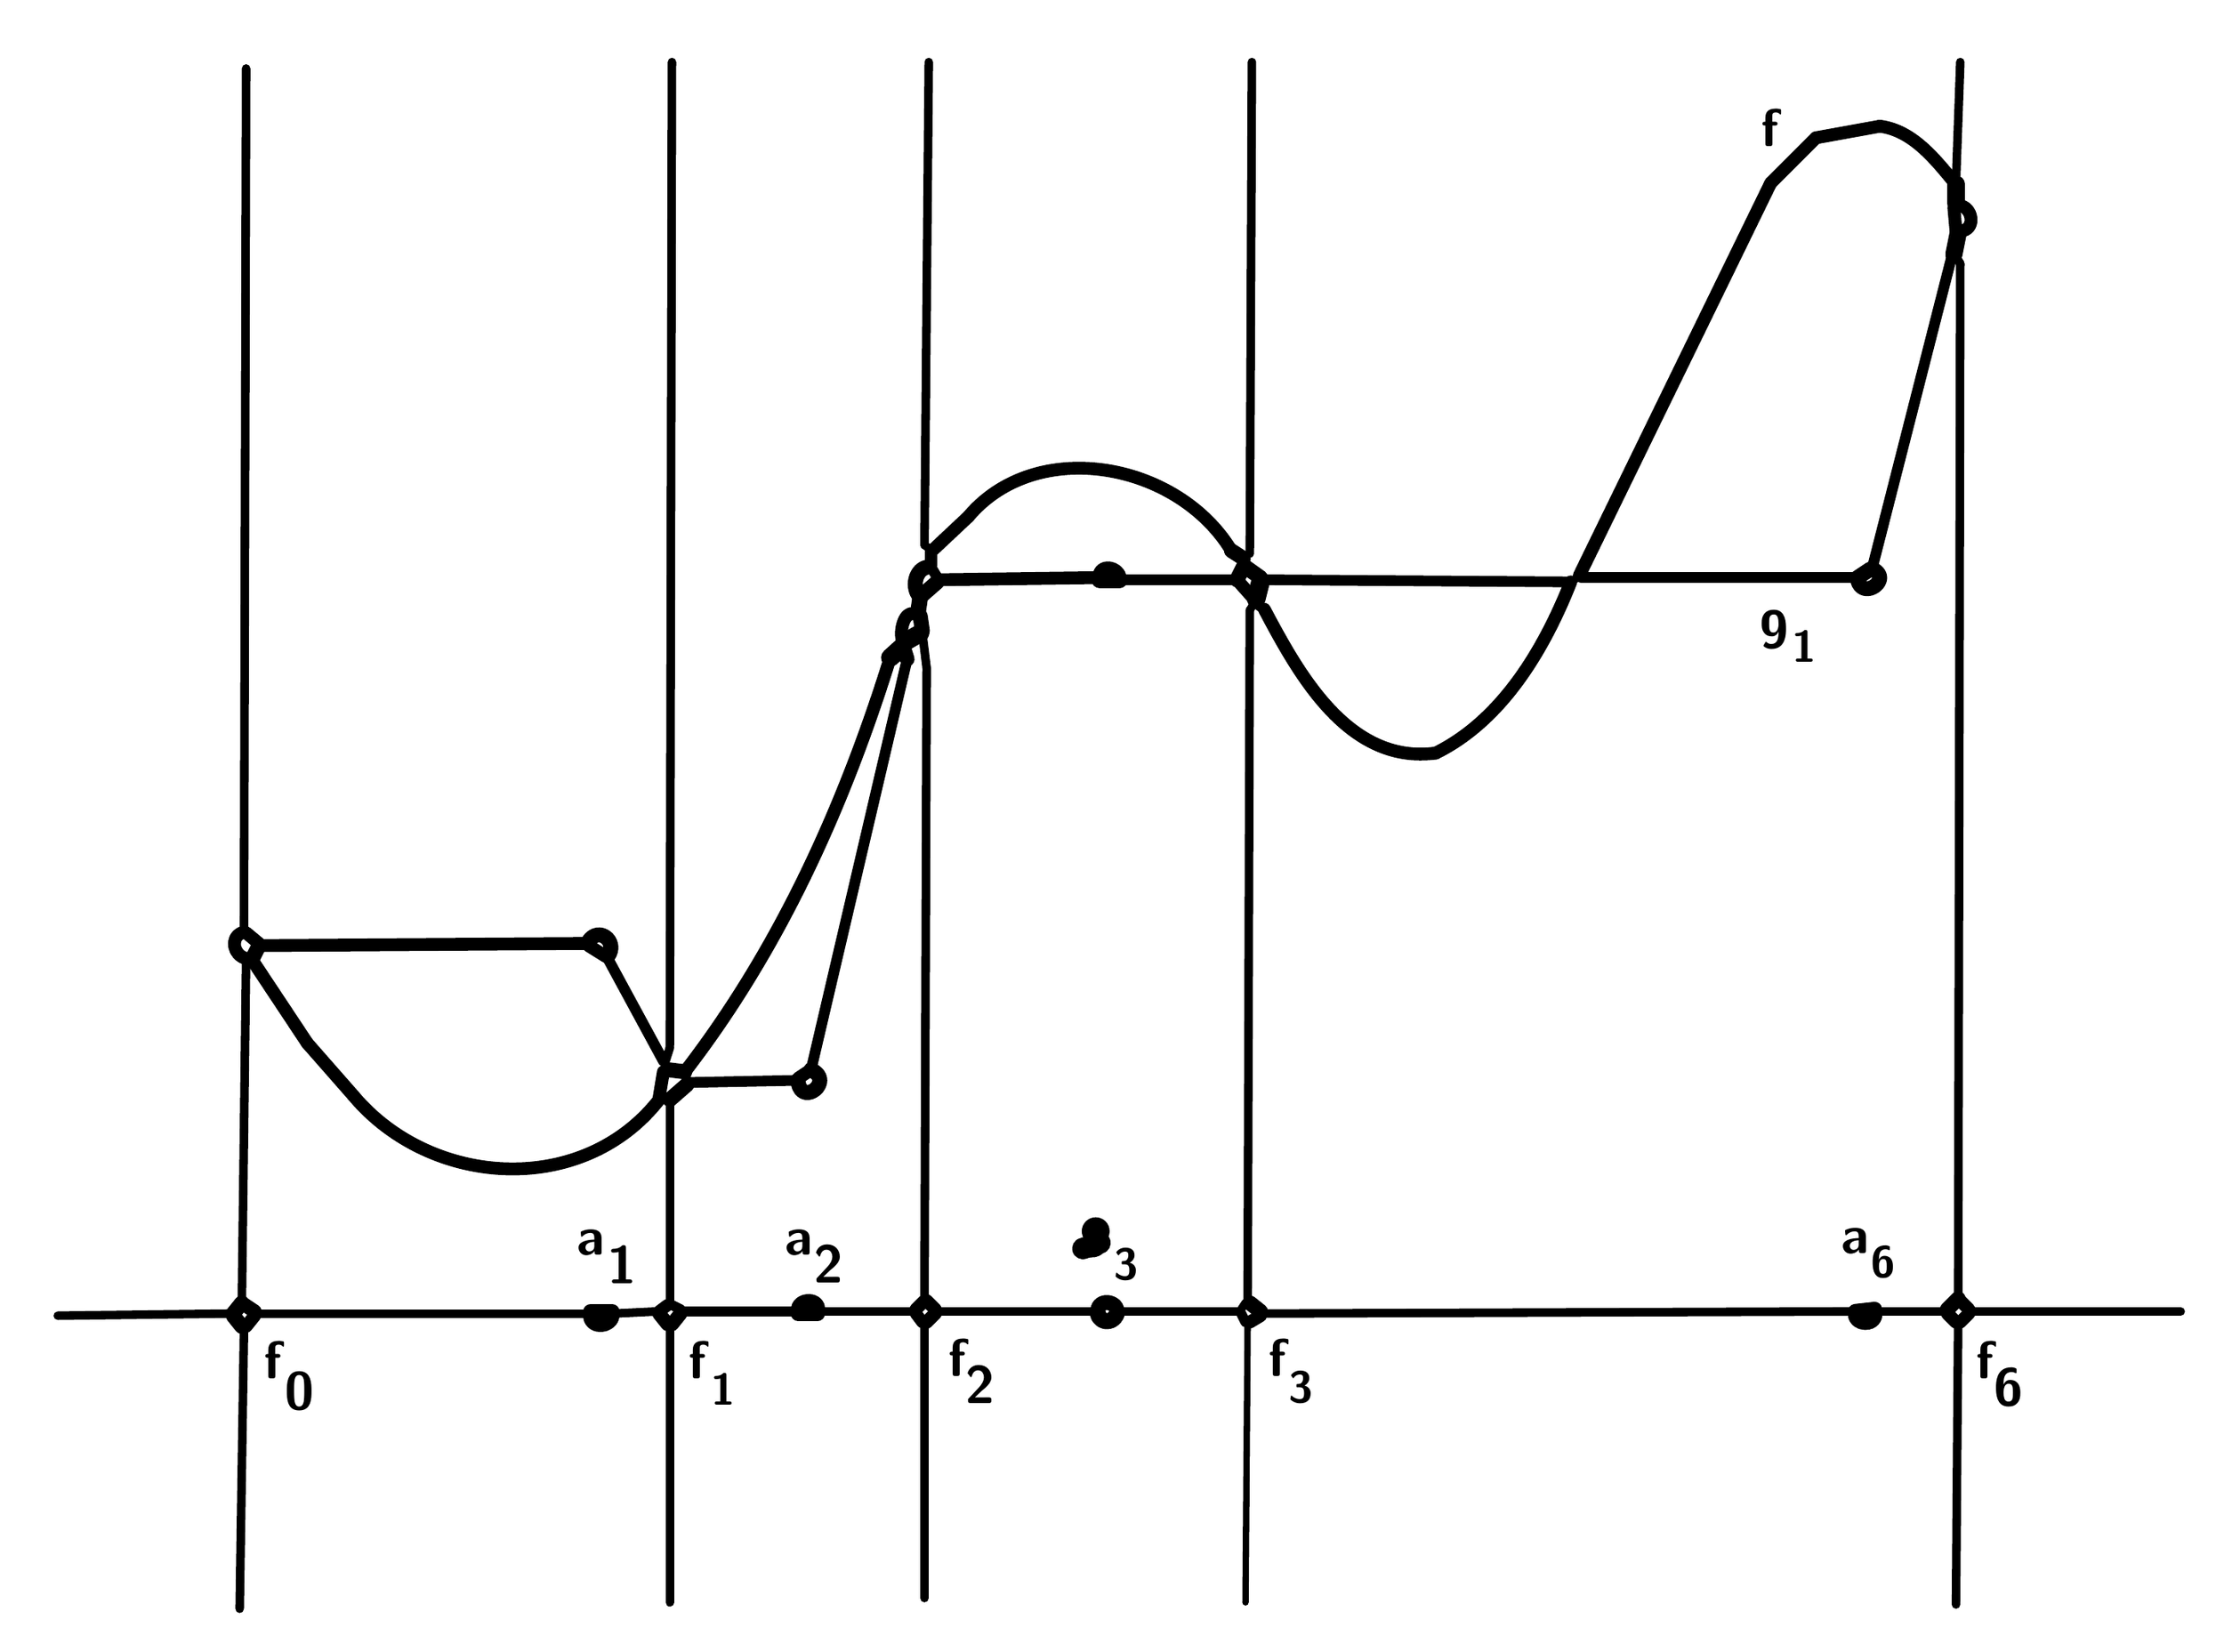
\begin{tikzpicture}[x=1pt, y=-1pt, line width=5.0pt, line cap=round, line join=round]

  %% ════ 填充区（prims2 的 fills）════

  %% ════ 直线段（prims2 的 strokes）════
  \draw[line width=5.0pt] (580.0,261.0) -- (724.0,262.0);
  \draw[line width=8.7pt] (579.0,262.0) -- (577.0,270.0);
  \draw[line width=6.0pt] (910.0,604.0) -- (906.0,608.0);
  \draw[line width=4.0pt] (1009.0,603.0) -- (911.0,603.0);
  \draw[line width=5.7pt] (302.0,600.0) -- (298.0,603.0);
  \draw[line width=4.0pt] (899.0,603.0) -- (867.0,603.0);
  \draw[line width=4.0pt] (417.0,603.0) -- (373.0,603.0);
  \draw[line width=5.0pt] (312.0,496.0) -- (362.0,495.0);
  \draw[line width=5.0pt] (362.0,603.0) -- (309.0,603.0);
  \draw[line width=6.0pt] (109.0,605.0) -- (105.0,610.0);
  \draw[line width=5.0pt] (369.0,490.0) -- (413.9,298.1);
  \draw[line width=6.9pt] (413.9,298.1) -- (412.0,292.0);
  \draw[line width=6.0pt] (369.0,490.0) -- (363.0,494.0);
  \draw[line width=4.0pt] (856.0,603.0) -- (580.0,604.0);
  \draw[line width=6.1pt] (423.0,598.0) -- (427.0,602.0);
  \draw[line width=4.0pt] (303.0,599.0) -- (303.0,505.0);
  \draw[line width=6.0pt] (576.0,270.0) -- (568.0,261.0);
  \draw[line width=4.0pt] (110.0,604.0) -- (265.0,604.0);
  \draw[line width=3.8pt] (727.0,260.0) -- (724.0,262.0);
  \draw[line width=3.0pt] (572.0,251.0) -- (574.0,248.8);
  \draw[line width=4.0pt] (574.0,248.8) -- (575.0,19.0);
  \draw[line width=6.0pt] (903.0,87.0) -- (904.0,98.0);
  \draw[line width=6.0pt] (264.0,431.0) -- (112.0,432.0);
  \draw[line width=6.0pt] (298.0,503.0) -- (300.0,491.0);
  \draw[line width=3.8pt] (576.0,272.0) -- (574.0,275.2);
  \draw[line width=4.0pt] (574.0,275.2) -- (573.0,598.0);
  \draw[line width=4.0pt] (304.0,19.0) -- (303.0,479.8);
  \draw[line width=4.0pt] (303.0,479.8) -- (301.0,486.0);
  \draw[line width=4.0pt] (428.0,603.0) -- (502.0,603.0);
  \draw[line width=6.0pt] (111.0,431.0) -- (105.0,426.0);
  \draw[line width=6.0pt] (429.0,261.0) -- (503.0,260.0);
  \draw[line width=7.0pt] (428.0,262.0) -- (420.0,269.0);
  \draw[line width=7.0pt] (266.0,603.0) -- (276.0,603.0);
  \draw[line width=6.0pt] (273.0,437.0) -- (265.0,432.0);
  \draw[line width=5.0pt] (729.0,260.0) -- (857.0,260.0);
  \draw[line width=5.0pt] (425.0,255.0) -- (428.0,260.0);
  \draw[line width=7.0pt] (420.0,278.0) -- (421.0,285.0);
  \draw[line width=4.0pt] (303.0,739.0) -- (303.0,610.0);
  \draw[line width=3.0pt] (299.0,504.0) -- (302.0,504.0);
  \draw[line width=4.0pt] (421.0,286.0) -- (423.0,302.2);
  \draw[line width=4.0pt] (423.0,302.2) -- (422.0,597.0);
  \draw[line width=8.0pt] (904.0,76.0) -- (904.0,85.0);
  \draw[line width=7.0pt] (571.0,255.0) -- (568.0,261.0);
  \draw[line width=8.0pt] (504.0,261.0) -- (513.0,261.0);
  \draw[line width=5.0pt] (568.0,261.0) -- (514.0,261.0);
  \draw[line width=8.6pt] (406.0,297.4) -- (412.0,292.0);
  \draw[line width=7.0pt] (310.0,491.0) -- (302.0,490.0);
  \draw[line width=4.3pt] (310.0,491.0) -- (311.0,495.0);
  \draw[line width=5.0pt] (274.0,438.0) -- (300.0,486.0);
  \draw[line width=6.0pt] (910.0,602.0) -- (905.0,597.0);
  \draw[line width=5.0pt] (902.0,110.0) -- (865.0,255.0);
  \draw[line width=6.0pt] (579.0,605.0) -- (574.0,608.0);
  \draw[line width=6.5pt] (302.0,609.0) -- (298.0,604.0);
  \draw[line width=7.0pt] (579.0,603.0) -- (574.0,599.0);
  \draw[line width=3.8pt] (572.0,599.0) -- (570.0,602.0);
  \draw[line width=4.0pt] (102.0,742.0) -- (104.0,611.0);
  \draw[line width=7.0pt] (864.0,256.0) -- (858.0,260.0);
  \draw[line width=6.1pt] (904.0,608.0) -- (900.0,604.0);
  \draw[line width=4.0pt] (98.0,604.0) -- (17.0,605.0);
  \draw[line width=5.7pt] (418.0,604.0) -- (421.0,608.0);
  \draw[line width=7.0pt] (363.0,604.0) -- (372.0,604.0);
  \draw[line width=4.0pt] (904.0,110.0) -- (906.0,113.2);
  \draw[line width=4.0pt] (906.0,113.2) -- (905.0,597.0);
  \draw[line width=6.5pt] (308.0,604.0) -- (304.0,609.0);
  \draw[line width=6.2pt] (427.0,604.0) -- (423.0,608.0);
  \draw[line width=7.0pt] (99.0,605.0) -- (103.0,610.0);
  \draw[line width=7.0pt] (866.0,602.0) -- (857.0,603.0);
  \draw[line width=7.0pt] (303.0,504.0) -- (311.0,497.0);
  \draw[line width=4.7pt] (304.0,600.0) -- (308.0,602.0);
  \draw[line width=3.0pt] (572.0,739.0) -- (573.0,609.0);
  \draw[line width=6.9pt] (571.0,251.0) -- (565.4,247.4);
  \draw[line width=6.0pt] (442.5,231.5) -- (426.0,247.0);
  \draw[line width=4.0pt] (103.0,599.0) -- (105.0,439.0);
  \draw[line width=7.0pt] (103.0,599.0) -- (99.0,604.0);
  \draw[line width=6.5pt] (103.0,599.0) -- (109.0,603.0);
  \draw[line width=6.0pt] (868.4,49.0) -- (838.6,54.4);
  \draw[line width=6.0pt] (838.6,54.4) -- (817.4,75.6);
  \draw[line width=6.0pt] (817.4,75.6) -- (728.0,259.0);
  \draw[line width=6.0pt] (108.0,439.0) -- (133.6,477.6);
  \draw[line width=6.0pt] (133.6,477.6) -- (155.1,502.1);
  \draw[line width=4.0pt] (512.0,603.0) -- (569.0,603.0);
  \draw[line width=4.0pt] (904.0,740.0) -- (905.0,609.0);
  \draw[line width=4.0pt] (906.0,19.0) -- (904.0,75.0);
  \draw[line width=4.0pt] (424.0,19.0) -- (422.0,244.8);
  \draw[line width=3.8pt] (422.0,244.8) -- (425.0,247.0);
  \draw[line width=4.0pt] (105.0,22.0) -- (104.0,425.0);
  \draw[line width=7.0pt] (900.0,602.0) -- (905.0,597.0);
  \draw[line width=6.0pt] (418.0,602.0) -- (422.0,598.0);
  \draw[line width=8.0pt] (903.0,109.0) -- (905.0,99.0);
  \draw[line width=4.0pt] (297.0,603.0) -- (277.0,604.0);
  \draw[line width=4.7pt] (570.0,604.0) -- (572.0,608.0);
  \draw[line width=4.9pt] (580.8,274.8) -- (577.0,272.0);
  \draw[line width=6.0pt] (425.0,248.0) -- (425.0,254.0);
  \draw[line width=7.3pt] (420.0,269.0) -- (419.0,276.0);
  \draw[line width=7.0pt] (111.0,432.0) -- (108.0,438.0);
  \draw[line width=8.4pt] (420.0,286.0) -- (413.0,290.0);
  \draw[line width=4.0pt] (422.0,737.0) -- (422.0,609.0);
  \draw[line width=7.0pt] (572.0,255.0) -- (579.0,260.0);
  \draw[line width=10.0pt] (504.0,571.0) -- (496.0,573.6);

  %% ════ 曲线（prims2 的 curves —— 三段式，坐标同为 (y,x)）════
  \draw[line width=7.0pt] (369.0,490.0) .. controls (380.3,495.2) and (364.8,507.4) .. (363.0,496.0);
  \draw[line width=6.0pt] (105.0,438.0) .. controls (99.2,436.7) and (97.2,428.5) .. (103.0,426.0);
  \draw[line width=7.0pt] (857.0,604.0) .. controls (856.5,609.4) and (866.8,609.7) .. (866.0,604.0);
  \draw[line width=7.5pt] (503.0,604.0) .. controls (504.3,609.5) and (511.6,608.3) .. (512.0,603.0);
  \draw[line width=6.0pt] (412.0,290.0) .. controls (409.8,286.3) and (412.4,275.2) .. (417.0,277.0);
  \draw[line width=6.0pt] (310.0,491.0) .. controls (354.8,433.0) and (384.7,365.9) .. (406.0,297.4);
  \draw[line width=7.0pt] (503.0,602.0) .. controls (503.9,597.1) and (512.0,598.2) .. (512.0,603.0);
  \draw[line width=6.0pt] (565.4,247.4) .. controls (540.2,205.8) and (474.1,193.9) .. (442.5,231.5);
  \draw[line width=7.0pt] (265.0,430.0) .. controls (270.0,422.6) and (279.0,430.4) .. (274.0,437.0);
  \draw[line width=7.0pt] (266.0,605.0) .. controls (265.9,610.8) and (275.4,610.2) .. (276.0,605.0);
  \draw[line width=6.0pt] (903.0,75.0) .. controls (893.9,64.0) and (883.5,50.9) .. (868.4,49.0);
  \draw[line width=7.0pt] (504.0,259.0) .. controls (504.8,254.0) and (512.2,255.6) .. (513.0,260.0);
  \draw[line width=7.0pt] (858.0,261.0) .. controls (860.4,271.0) and (874.7,260.5) .. (865.0,256.0);
  \draw[line width=6.0pt] (155.1,502.1) .. controls (191.3,545.3) and (262.4,549.6) .. (298.0,504.0);
  \draw[line width=7.0pt] (424.0,255.0) .. controls (417.6,255.5) and (415.7,265.0) .. (420.0,269.0);
  \draw[line width=7.0pt] (363.0,602.0) .. controls (363.4,597.3) and (372.4,597.0) .. (372.0,602.0);
  \draw[line width=6.0pt] (724.0,262.0) .. controls (711.8,292.8) and (692.4,326.4) .. (660.9,342.0);
  \draw[line width=6.0pt] (660.9,342.0) .. controls (620.0,347.5) and (596.7,304.8) .. (580.8,274.8);
  \draw[line width=6.0pt] (905.0,86.0) .. controls (911.9,86.2) and (913.7,97.6) .. (906.0,98.0);
  \draw[line width=5.0pt] (496.0,573.6) .. controls (497.9,576.3) and (505.8,575.9) .. (504.0,571.0);

  %% ════ 实心点 ════
  \fill (502.0,565.5) circle (6.5);

  %% ════ 标签（probe 直接给的 \node 行）════
  %% ⚠ 全部补了 fill=white：文字在最上层，否则与曲线交叉干扰
     \node[anchor=center,inner sep=0pt,fill=white,font=\fontsize{29.1}{36.4}\selectfont] at (818.0,50.0) {\textsf{\textbf{\textit{f}}}};   % box(812,38,11,23)
     \node[anchor=center,inner sep=0pt,fill=white,font=\fontsize{34.8}{43.5}\selectfont] at (819.0,284.4) {\textsf{\textbf{9}}};   % box(808,272,18,23)
     \node[anchor=center,inner sep=0pt,fill=white,font=\fontsize{22.2}{27.8}\selectfont] at (833.1,292.4) {\textsf{\textbf{1}}};   % box(827,284,7,16)
     \node[anchor=center,inner sep=0pt,fill=white,font=\fontsize{32.0}{40.0}\selectfont] at (857.1,570.1) {\textsf{\textbf{\textit{a}}}};   % box(848,560,16,17)
     \node[anchor=center,inner sep=0pt,fill=white,font=\fontsize{32.0}{40.0}\selectfont] at (266.1,571.1) {\textsf{\textbf{\textit{a}}}};   % box(257,561,16,17)
     \node[anchor=center,inner sep=0pt,fill=white,font=\fontsize{31.0}{38.7}\selectfont] at (363.5,571.0) {\textsf{\textbf{\textit{a}}}};   % box(355,561,15,17)
     \node[anchor=center,inner sep=0pt,fill=white,font=\fontsize{23.6}{29.6}\selectfont] at (377.1,580.9) {\textsf{\textbf{2}}};   % box(371,572,11,17)
     \node[anchor=center,inner sep=0pt,fill=white,font=\fontsize{21.9}{27.4}\selectfont] at (516.4,581.0) {\textsf{\textbf{3}}};   % box(511,572,10,17)
     \node[anchor=center,inner sep=0pt,fill=white,font=\fontsize{22.0}{27.4}\selectfont] at (870.0,580.0) {\textsf{\textbf{6}}};   % box(864,572,11,15)
     \node[anchor=center,inner sep=0pt,fill=white,font=\fontsize{23.7}{29.7}\selectfont] at (280.8,581.4) {\textsf{\textbf{1}}};   % box(274,573,8,16)
     \node[anchor=center,inner sep=0pt,fill=white,font=\fontsize{26.5}{33.1}\selectfont] at (438.4,624.9) {\textsf{\textbf{\textit{f}}}};   % box(433,614,10,21)
     \node[anchor=center,inner sep=0pt,fill=white,font=\fontsize{25.2}{31.4}\selectfont] at (587.9,624.9) {\textsf{\textbf{\textit{f}}}};   % box(583,614,9,21)
     \node[anchor=center,inner sep=0pt,fill=white,font=\fontsize{26.5}{33.1}\selectfont] at (118.4,625.9) {\textsf{\textbf{\textit{f}}}};   % box(113,615,10,21)
     \node[anchor=center,inner sep=0pt,fill=white,font=\fontsize{25.2}{31.4}\selectfont] at (316.9,625.9) {\textsf{\textbf{\textit{f}}}};   % box(312,615,9,21)
     \node[anchor=center,inner sep=0pt,fill=white,font=\fontsize{26.5}{33.1}\selectfont] at (918.4,625.9) {\textsf{\textbf{\textit{f}}}};   % box(913,615,10,21)
     \node[anchor=center,inner sep=0pt,fill=white,font=\fontsize{22.9}{28.7}\selectfont] at (448.1,637.4) {\textsf{\textbf{2}}};   % box(442,629,11,16)
     \node[anchor=center,inner sep=0pt,fill=white,font=\fontsize{22.3}{27.9}\selectfont] at (597.9,638.6) {\textsf{\textbf{3}}};   % box(592,630,11,16)
     \node[anchor=center,inner sep=0pt,fill=white,font=\fontsize{23.7}{29.6}\selectfont] at (928.6,638.6) {\textsf{\textbf{6}}};   % box(922,630,12,16)
     \node[anchor=center,inner sep=0pt,fill=white,font=\fontsize{22.2}{27.8}\selectfont] at (328.1,639.4) {\textsf{\textbf{1}}};   % box(322,631,7,16)
     \node[anchor=center,inner sep=0pt,fill=white,font=\fontsize{24.1}{30.2}\selectfont] at (130.0,640.2) {\textsf{\textbf{0}}};   % box(122,632,12,16)

  % 钉死画布：否则超出的图元/控制点会把页面撑大，1:1 回比就失准
  \pgfresetboundingbox
  \path[use as bounding box] (0,0) rectangle (1019,752);
\end{tikzpicture}
\end{document}

% ⚠ 待核清单（probe 拿不准，人眼过一遍）：
%   · 未识别/跳过：⑤ 跳过/未识别的字形
